\section{Model Problems}

\subsection{Time-Dependent Advection Diffusion Models}

%%%%%%%%%%%%%%%%%%%%%%%%%%%%%%%%%%%%%%%%%%
\begin{frame}{SISO Notation}
Proposed system is single input (${\bf u}(t) \in \real$) and single output (${\bf z}(t) \in \real$)\\
\bigskip
Change of notation:\\
\bigskip
$\bA, {\bf E} \in \real^{n \times n}$, ${\bf b},{\bf c} \in \real^n$, and ${\bf d} \in \real$\\

\begin{align*}
            {\bf E}\frac{d}{dt} {\bf y}(t)  &= \bA {\bf y}(t) + {\bf b}{\bf u}(t)\\
            {\bf z}(t) &= {\bf c}^T {\bf y}(t) + {\bf d}{\bf u}(t)
\end{align*}


\end{frame}
%%%%%%%%%%%%%%%%%%%%%%%%%%%%%%%%%

\begin{frame}{1D Time-Dependent Advection Diffusion Equation}
	Partial differential equation (PDE):
	 \begin{align*}
                         \frac{\partial}{\partial t} y(x,t) 
                        - \alpha \frac{\partial^2}{\partial x^2} y(x,t) +  \beta \frac{\partial}{\partial x} y(x,t) &= 0
                                                & x \in (0,1), t \in (0,T), \\
                         y(0,t) &= u(t),    & t \in (0,T), \\
                         y_x(1,t) &= 0,    & t \in (0,T), \\
                         y(x,0) &= y_0(x),  & x \in (0,1),
          \end{align*}
          with $\alpha > 0$ and $\beta >0$. We use
         \[
                \alpha=0.01, \beta = 1, T=0.5.
          \]
        \begin{minipage}[c]{0.6\textwidth}
	Output:
	\[
	   z(t) = \int_{0}^{1} y(x,t) dx
	\]
	\end{minipage} \hfil
         \begin{minipage}[c]{0.35\textwidth}
	\begin{center}
               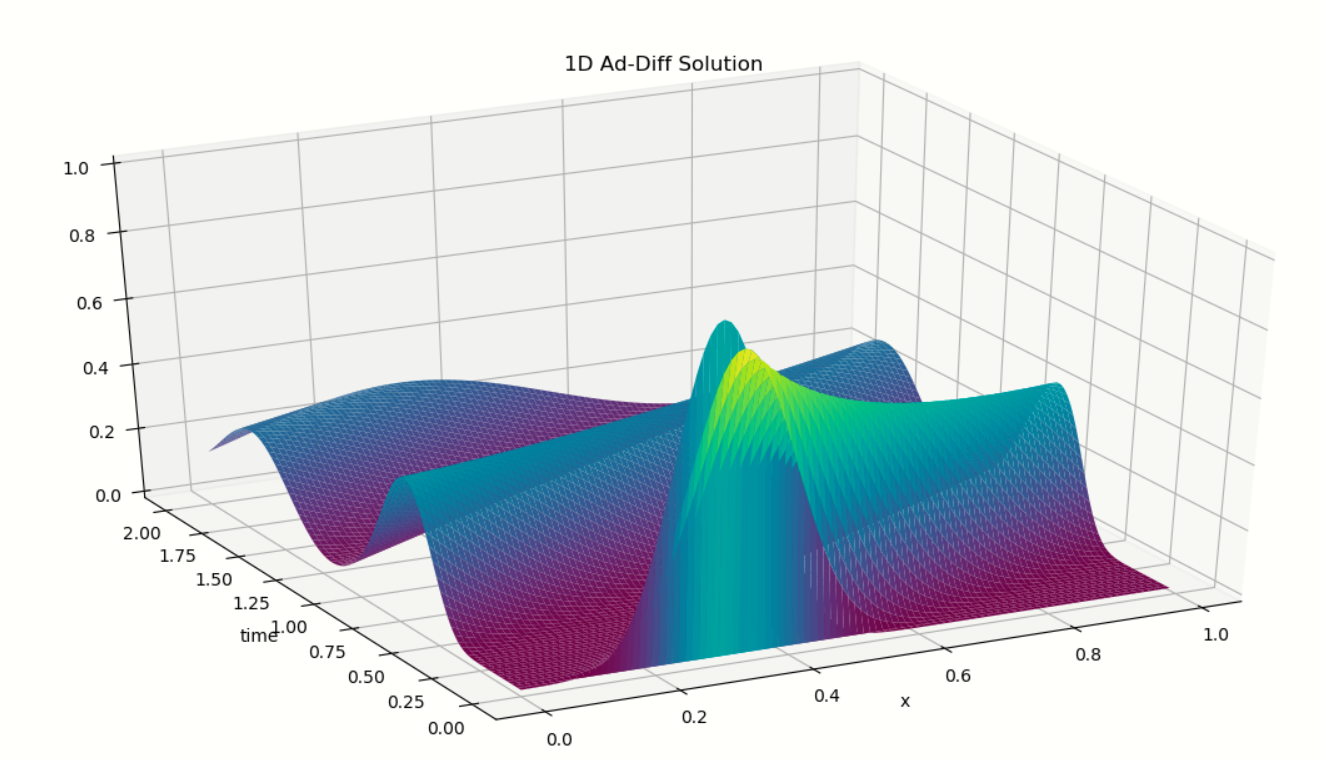
\includegraphics[width=1.0\textwidth]{figures/1D_addiffsol.PNG}\\
               PDE solution
	\end{center}
	\end{minipage}
\end{frame}


%%%%%%%%%%%%%%%%%%%%%%%%%%%%%%%%%%%%%%%%%%%%%%%%%%%%%%%%%%%%%%%%%%%%%%%%%%

\begin{frame}{1D Advection Diffusion Discretization}

Upwind finite difference discretization in space leads to
         \[
                    \frac{d}{dt} {\bf y}(t)  = \bA {\bf y}(t) + {\bf b}{\bf u}(t), \quad t \in (0,T), \qquad {\bf y}(0) = {\bf y}_0,
        \]
        where \({\bf A} = \alpha \bA^{diff} + \beta \bA^{conv}\)
        \begin{align*}
              \setlength{\arraycolsep}{2pt}
              \renewcommand{\arraystretch}{0.9}
              \bA^{diff} = \begin{bmatrix}
              -2 & 1\\
              1 & -2 & -1\\
              &   \ddots & \ddots & \ddots\\
              &   &     1 & -2 & 1\\
              &&& 2 & -2
              \end{bmatrix}
        &
              \setlength{\arraycolsep}{2pt}
              \renewcommand{\arraystretch}{0.9}
              \bA^{conv} = \begin{bmatrix}
              -1\\
              1 & -1 \\
              &   \ddots & \ddots\\
              &   &     1 & -1\\
              &&& 1 & -1
              \end{bmatrix}
        \end{align*}
        \[
             {\bf y}_0 =  \Big(y_0(x_0,t), \ldots,  y_0(x_{n_x-1},t) \Big)^T \in \real^{n_x}             
        \]
        
        \[
             {\bf b} =  \Big( \frac{\alpha}{h^{2}}+\frac{\beta}{h},0, \ldots,0 \Big)^T \in \real^{n_x}             
        \]

\end{frame}


%%%%%%%%%%%%%%%%%%%%%%%%%%%%%%%%%%%%%%%%%%%%%%%%%%%%%%%%%%%%%%%%%%%%%%%%%%%%%%%%%%%%

\begin{frame}{1D Advection Diffusion Discretization (cont.)}

Composite Trapezoidal Rule:
\begin{align*}
     \int_{0}^{1} y(x,t)dx & \approx \frac{h}{2} y(x_0,t) + hy(x_1,t) + \ldots + hy(x_{n_x -1},t) + \frac{h}{2} y(x_n,t)
     \\
     & = \frac{h}{2}u(t) + hy(x_1,t) + \ldots + hy(x_{n_x -1},t) + \frac{h}{2} y(x_n,t)\\
\end{align*}
    
Leads to:
\begin{align*}
     \int_{0}^{1} y(x,t)dx & \approx \frac{h}{2} u(t) + hy_1(t) + \ldots + hy_{n_x -1}(t) + \frac{h}{2} y_{n_x}(t)
     \\
     & = {\bf c}^{T} {\bf y}(t) + {\bf d}{\bf u}(t)\\
\end{align*}
with 
\begin{align*}
{\bf c} &=  \big( h,h,\ldots,h,\frac{h}{2} \big)^{T} \in \real^{n_x}\\
{\bf d} &= \frac{h}{2}
\end{align*}

\end{frame}

%%%%%%%%%%%%%%%%%%%%%%%%%%%%%%%%%%%%%%%%%%%%%%%%%%%%%%%%%%%%%%%%%%%%%%%%%%
\subsection{Laplace Transform}

\begin{frame}{Laplace Transform}
Transforms a function of time to function of a frequency\\
\bigskip
Let $q(t)$ be function of time where $t \in \real$\\
\bigskip
Denote $\mathcal{L}(q)$ as $q(s)$ where $s \in \mathbb{C}$ is frequency
\end{frame}
%%%%%%%%%%%%%%%%%%%%%%%%%%%%%%%%%%%%%%%%%%%%%%%%%%%%%%%
\begin{frame}{Laplace Transform}

Apply the Laplace Transform to the system:
    \begin{align*}
            {\bf E}\frac{d}{dt} {\bf y}(t)  = \bA {\bf y}(t) + {\bf b}{\bf u}(t)\\
            {\bf z}(t) = {\bf c}^T {\bf y}(t) + {\bf d}{\bf u}(t)
    \end{align*}
\\
which turns into:
\\
    \begin{align*}
        s{\bf E} {\bf y}(s) - {\bf y}(0) &= {\bf A} {\bf y}(s) + {\bf b}{\bf u}(s)\\
        {\bf z}(s) &= {\bf c}^T {\bf y}(s) + {\bf d} {\bf u}(s)
    \end{align*}

\end{frame}
%%%%%%%%%%%%%%%%%%%%%%%%%%%%%%%%%%%%%%%%%%%%%%%%%%%%%%%%%%%%%%%%%%%%%%%%%%%%%%%%%%%%%%%%%%%%%%%%%%%%%%%%%%%%%

\begin{frame}{Laplace Transform}
Assume ${\bf y}(0) = 0$\\
\bigskip
Rearrange and solve:
    \begin{align*}
        {\bf y}(s) &= \Big(\Big( s{\bf E} - {\bf A} \Big)^{-1} {\bf b} \Big) {\bf u}(s)
    \end{align*}
Substitute to get:
    \begin{align*}
        {\bf z}(s) &=  \Big( {\bf c}^T \Big(s{\bf E} - {\bf A} \Big)^{-1} {\bf b} + {\bf d} \Big) {\bf u}(s)
    \end{align*}

 Which gives the following transfer function ${\bf H}(s)$:
    \begin{align*}
        {\bf H}(s) &= {\bf c}^T \Big( s{\bf E}- {\bf A} \Big)^{-1} {\bf b} + {\bf d}, \quad s \in \mathbb{C}\\
    \end{align*}
\end{frame}
%%%%%%%%%%%%%%%%%%%%%%%%%%%%%%%%%%%%%%%%%%%%%%%%%%%%%%%%%%%%%
\begin{frame}{1D Advection Diffusion Transfer Function}
    \centering
    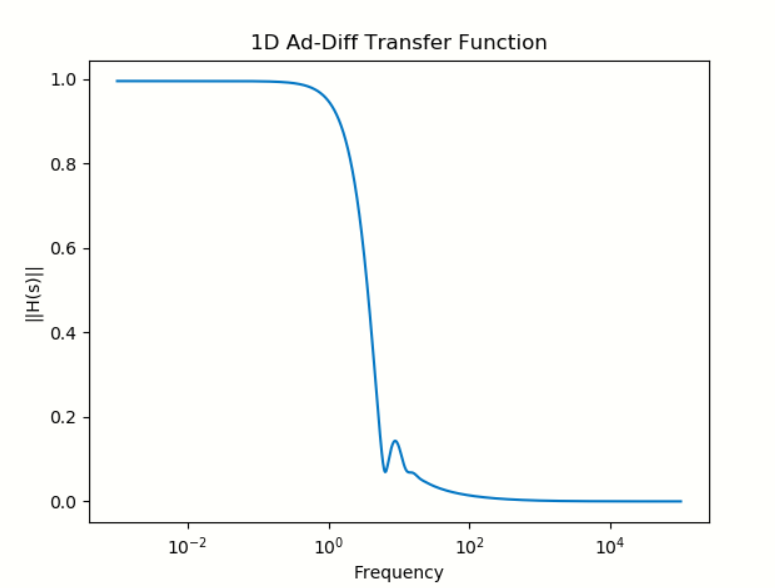
\includegraphics[width=7cm, height=5cm]{figures/1d_transfer.PNG}
\end{frame}